% 研究会 卒論概要（2段組み1〜2ページ）
% ビルド: platex gaiyou.tex && platex gaiyou.tex && dvipdfmx gaiyou.dvi
%
% 【確定事項（2026-10-13）】
%   学籍番号 922086 ／ 題目は outline.md の仮題目のままで可 ／
%   機体写真は載せない（周知のため不要との判断）
%
% 【数値の出所】すべて docs/thesis/ の実データ．創作値は無い．
%   表1・本文の数値 = 表5.10 / 表6.3（2026-07-15 実機バッチ・n=3）
%   図1 = results/2026-07-26_thesis_figs/fig5_6_omega_before_after.png（各代表1本）
%   注意: 図1 のキャプション内数値は代表1本、本文・表1 は n=3 平均なので僅かに違う
\documentclass[a4jsme,9pt,dvipdfmx]{jsmepaper_robomec}
\usepackage{epic,eepic}
\usepackage{graphicx}
\usepackage{bm}
\usepackage{url}
\usepackage{here}
\usepackage{caption}
\usepackage[top=25truemm,bottom=30truemm,left=20truemm,right=16truemm,headsep=0mm]{geometry}
\usepackage{fancyhdr}
\usepackage{subfigure}
\usepackage{amsmath}
\usepackage{ascmac}
\pagestyle{empty}
\newlength{\minitwocolumn}
\renewcommand{\refname}{参考文献}
\renewcommand{\baselinestretch}{1}
\setlength{\columnsep}{4zw}

\jtitle{\Large{農業用ロボットの経路追従におけるスパース最適制御の実機適用}}
\jauthor{
         \large{向川 航平（922086）\hspace{27pt}指導教員：小野山 博之}
     }
\date{}
\keywords{}
\abstract{
\vspace{-6mm}
}

\begin{document}
\maketitle
\thispagestyle{fancy}
\renewcommand{\headrulewidth}{0pt}
\lhead{}
\rhead{}
\cfoot{}
\small{}

\section{研究目的}
農業分野では担い手の減少と高齢化が進んでいる．
農林水産省の農林業センサスによれば，基幹的農業従事者は令和2年の136.3万人から
令和7年の103.6万人へと5年間で24.0\,\%減少し，平均年齢は67.7歳，
65歳以上が69.6\,\%を占める\cite{maff}．
この状況に対し農業機械の自動化が求められており，その基盤となるのが経路追従制御である．

従来の経路追従手法は，追従誤差に応じて操舵量を連続的に決める．
Kanayamaらの制御則\cite{kanayama}も標準的なモデル予測制御（MPC）も，
誤差がゼロでない限り何らかの入力を出し続けるため，
\textbf{機体は微小な誤差に対しても常時操舵し続ける}．
これはアクチュエータの消耗を招き，滑りやすい路面では細かな操舵が滑りを誘発しうる．

ここから「必要なときにだけ大きく動かし，それ以外は完全に止めておけないか」という問いが立つ．
この問いに対する枠組みが永原による\textbf{最大ハンズオフ制御}\cite{nagahara,nagahara-tac}であり，
入力の大きさではなく\textbf{入力がちょうどゼロである時間を最大化する}設計論である．
本研究はこの設計論を\textbf{実機の経路追従に持ち込む}ことを目的とする．
シミュレーション上での有効性は既に示されているが，
計算資源の限られた実機に載せたときに何が起きるかは自明ではない．

\section{提案手法}
誤差ダイナミクスを参照軌道まわりで線形化し，MPCの評価関数の入力項を
$L^2$ から $L^1$ へ置き換える（$L^1$-MPC）．$L^1$ 最小化は凸最適化として解け，
その解は入力が上限・下限・ゼロのいずれかを取る bang-off-bang 構造をもつ．

しかし\textbf{これを実機に載せると，曲線経路のコーナーで激しいチャタリングが生じた．}
入力の総量はベースラインの4.1倍に達し，ゼロ入力率は全手法中で最低となった．
この現象はシミュレーションでは再現されず，遅延注入シミュレーションにより
\textbf{原因が実機の入力遅延（約200\,ms，制御周期2ステップ相当）であること}を特定した．
遅延下では符号が反転したあとに状態が追従せず，次の時刻で逆向きの飽和入力が選ばれ続ける．

そこで対策として，入力の\textbf{変化率}にペナルティを与える移動抑制項を評価関数に加える．
\begin{equation}
  \begin{split}
    \min_{\delta u} \ & \sum_{k=0}^{N-1} \left( \|z_k\|_Q^2
      + \lambda \|\delta u_k\|_1
      + w_{ms} \|\delta u_k - \delta u_{k-1}\|^2 \right) + \|z_N\|_{Q_f}^2 \\
    \mathrm{s.t.} \ & z_{k+1} = A z_k + B \delta u_k, \quad
      |u_{\mathrm{ref}} + \delta u_k| \le u_{\max}
  \end{split}
\end{equation}
ここで $z$ は追従誤差，$\delta u$ は参照速度からの補正入力，
$\lambda$ は $L^1$ 項の重み，$w_{ms}$ は移動抑制の重みである．
$L^1$ ペナルティを補正入力 $\delta u$ に課すことで，
巡航を維持したまま\textbf{補正を打つ瞬間だけ動かす}スパース操舵が得られる．
$L^1$ 項がゼロを生む作用を保ったまま，連続する入力の飛びだけを抑える狙いである．

\section{システム概要}
対象は差動二輪型の小型移動ロボット LiteRover（ヴィストン製）である．
車載計算機は Raspberry Pi 4 であり，
\textbf{計算資源の限られた実機の上で制御則を実時間で解く}ことが前提となる．
制御周期は10\,Hz，予測ホライズンは $N=15$ とした．
凸最適化ソルバには OSQP を用い，前時刻の解を初期値とする warm start により
求解時間を抑えている．$N\le30$ であれば制御周期内に求解できることを実機で確認した．

\section{実験方法}
屋内の平坦な床面に1.5\,m四方のL字経路を設定し，
Kanayama則・$L^2$-MPC・素の $L^1$-MPC・$L^1$-MPC＋移動抑制（提案手法）の
4条件を各3走行ずつ比較した．参照速度は一定とし，$\lambda=0.3$，$w_{ms}=2.0$ とした．

評価指標は，追従精度としての横偏差RMSE（オドメトリ基準），
操舵量 $\Sigma|u|$，振動の直接的な指標である $\omega$ の符号反転回数，
および $|\omega|<0.05$\,rad/s であった時間の割合（ゼロ入力率）である．

\section{実験結果}
結果を表\ref{tab:result}に示す（$n=3$，平均$\pm$標本標準偏差）．

\begin{center}
    \captionof{table}{実機バッチの結果（$n=3$）}
    \label{tab:result}
    \begin{tabular}{lcccc}
      \hline
      条件 & RMSE [cm] & $\Sigma|u|$ & 符号反転 & ゼロ率 \\
      \hline
      Kanayama       & 11.26 & 4.86 & 0 & 0.650 \\
      $L^2$-MPC      & \textbf{1.83} & \textbf{4.65} & 0 & 0.872 \\
      $L^1$（素）     & 3.49 & 19.17 & 18 & 0.529 \\
      提案手法        & 2.20 & 5.02 & 1 & \textbf{0.882} \\
      \hline
    \end{tabular}
\end{center}

素の $L^1$ は符号反転18回，$\Sigma|u|=19.17$，飽和率37\,\%でチャタリングしている．
移動抑制の導入により\textbf{符号反転は1回，$\Sigma|u|$ は5.02へ低下し，チャタリングは消失した}．
$\omega(t)$ の波形で見ると，同一のコーナーが
\textbf{上限への18回の往復から1回のなめらかな旋回へ変わる}（図\ref{fig:omega}）．

\begin{center}
    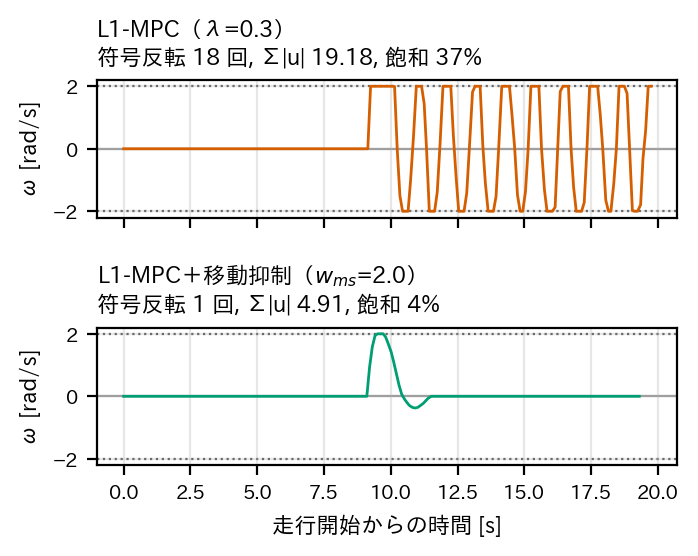
\includegraphics[width=0.98\linewidth]{fig/omega_before_after.png}
    \captionof{figure}{移動抑制の導入によるチャタリングの消失（各代表1本）}
    \label{fig:omega}
\end{center}

ここで最も重要なのは，\textbf{チャタリングを消してもスパース性が失われていない}ことである．
提案手法のゼロ入力率は0.882で，$L^2$-MPCの0.872を上回り4条件中で最良である．
すなわち移動抑制は「ゼロの多さ」を犠牲にせず「暴れ」だけを除いている．

\section{おわりに}
スパース最適制御を実機の経路追従へ適用し，
\textbf{$L^1$-MPCが実機の入力遅延下でチャタリングを起こすこと}を実機で提示したうえで，
入力変化率へのペナルティによりこれを消去できることを示した．
本研究の寄与は，シミュレーションで有効な設計が実機で成立しない理由を特定し，
その\textbf{成立条件}を示した点にある．
なお追従精度と計算負荷では $L^2$-MPC が最良であり，
提案手法が上回るのはゼロ入力率と最終姿勢精度である．
今後は積載外乱下での評価と，消費電力の直接計測による検証を行う．

\begin{thebibliography}{9}
  \bibitem{maff} 農林水産省：``農業労働力に関する統計''，農林業センサス，
    \url{https://www.maff.go.jp/j/tokei/sihyo/data/08.html}（参照 2026-10-13）
  \bibitem{kanayama} Y. Kanayama, Y. Kimura, F. Miyazaki and T. Noguchi:
    ``A stable tracking control method for an autonomous mobile robot'',
    Proc. IEEE ICRA, pp. 384-389 (1990)
  \bibitem{nagahara} 永原 正章：``最適制御とスパースモデリング''，
    電子情報通信学会 基礎・境界ソサイエティ Fundamentals Review，
    Vol. 10，No. 3，pp. 176-185 (2017)
  \bibitem{nagahara-tac} M. Nagahara, D. E. Quevedo and D. Ne\v{s}i\'{c}:
    ``Maximum hands-off control: a paradigm of control effort minimization'',
    IEEE Trans. Automatic Control, Vol. 61, No. 3, pp. 735-747 (2016)
\end{thebibliography}

\end{document}
